\subsection{Approach}
\label{sec:hard_cut_approach}

Hard cuts are abrupt transitions from one scene to another.
Normally the contents of the two frames involved in such a cut are highly different, see Figure~\ref{fig:hard_cut_example}, while two consecutive frames in one scene do not differ that much.

\begin{figure}[ht]
	\centering
	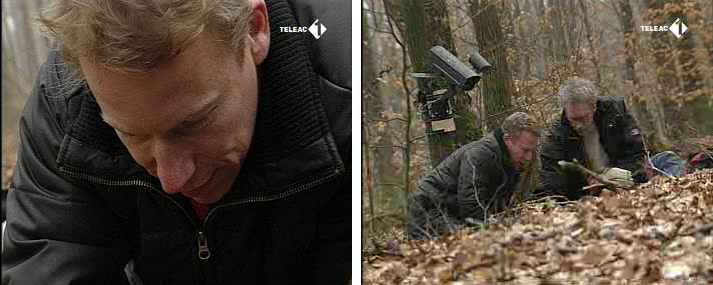
\includegraphics[scale=.5]{images/hard_cut_example.png}
	\caption{These two consecutive frames form a hard cut.}
	\label{fig:hard_cut_example}
\end{figure}

To detect hard cuts, we therefore want to apply a similarity measure to two subsequent frames.
In our case, we represent frames using their color histograms.
Each frame has three color channels (red, green, blue) and therefore three histograms.
The difference between two frames is then the difference between the histograms.
The histogram difference can be represented as a \emph{3*n}-dimensional vector, where \emph{n} is the number of bins in a color histogram.
So, we are presented with a binary classification task (cut or not) in a \emph{3*n}-dimensional space.

In a next step, the dimensionality can be further reduced by simply adding up the vector elements.
This step is justifiable, since it does not matter which color changed and how much, but the sum of changes in all color channels does.
Our results with the reduced dimensionality were better than those of the high dimensional approach.
That's why we use the latter.

To do the actual classification we train an SVM classifier on a labeled training set.
In our implementation, we use the SVM provided by the OpenCV library\footnote{\url{http://docs.opencv.org/doc/tutorials/ml/introduction_to_svm/introduction_to_svm.html}}.
We transform the input space into a higher dimensional feature space by using a kernelized decision function. The commonly used radial basis function (RBF) kernel is employed:
$$K(x_i,x_j) = exp(-\lambda || x_i - x_j ||^2)$$
where $\lambda$ denotes the width of the kernel and $x_i, x_j $ are vectors from the training set.
This is part of the library.
The complexity parameter C for the soft-margin SVM, as well as other parameters are optimized automatically by using the \emph{train\_auto} method of OpenCVs SVM implementation.
It automatically performs a k-fold cross-validation to choose the best parameter values.
